% Created by tikzDevice version 0.12.3.1 on 2023-04-07 11:09:53
% !TEX encoding = UTF-8 Unicode
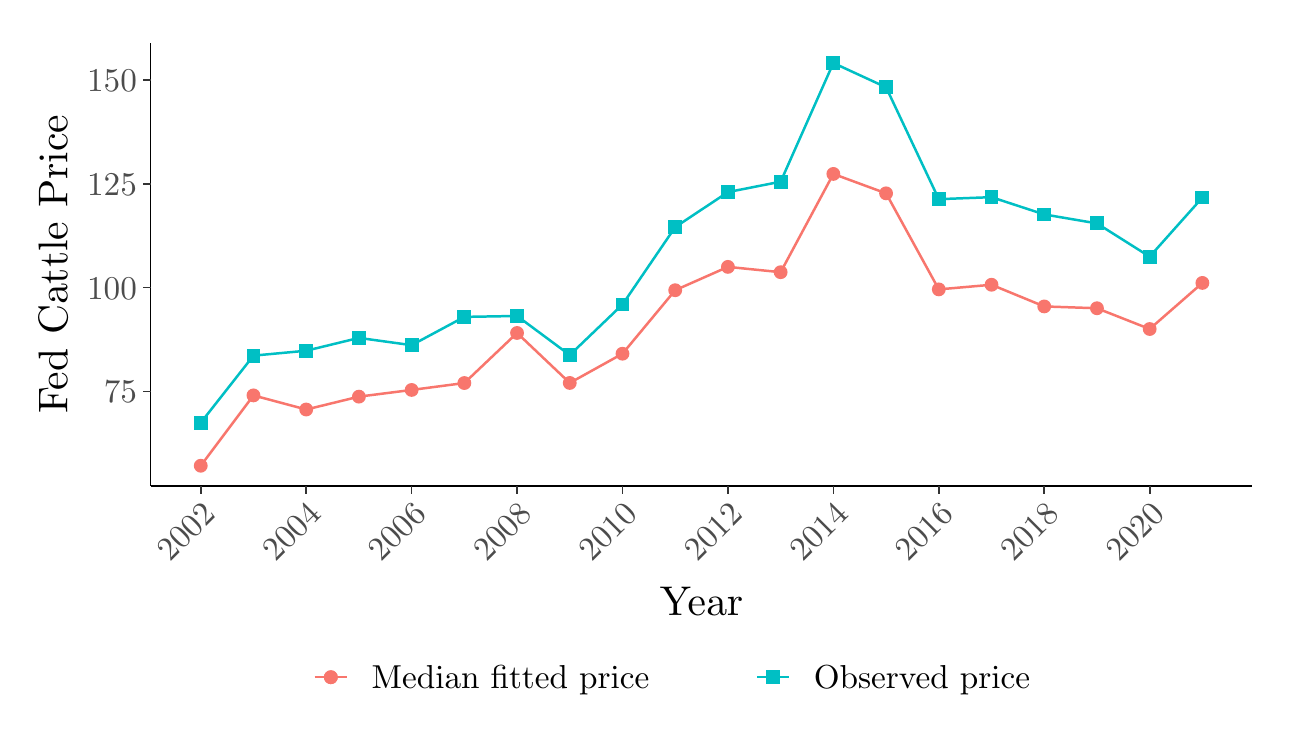
\begin{tikzpicture}[x=1pt,y=1pt]
\definecolor{fillColor}{RGB}{255,255,255}
\path[use as bounding box,fill=fillColor,fill opacity=0.00] (0,0) rectangle (448.07,252.94);
\begin{scope}
\path[clip] (  0.00,  0.00) rectangle (448.07,252.94);
\definecolor{drawColor}{RGB}{255,255,255}
\definecolor{fillColor}{RGB}{255,255,255}

\path[draw=drawColor,line width= 0.6pt,line join=round,line cap=round,fill=fillColor] (  0.00,  0.00) rectangle (448.07,252.94);
\end{scope}
\begin{scope}
\path[clip] ( 44.44, 87.36) rectangle (442.57,247.45);
\definecolor{fillColor}{RGB}{255,255,255}

\path[fill=fillColor] ( 44.44, 87.36) rectangle (442.57,247.44);
\definecolor{drawColor}{RGB}{0,191,196}

\path[draw=drawColor,line width= 0.9pt,line join=round] ( 62.54,110.18) --
	( 81.59,134.43) --
	(100.64,136.20) --
	(119.69,140.84) --
	(138.74,138.21) --
	(157.79,148.43) --
	(176.84,148.76) --
	(195.88,134.64) --
	(214.93,152.90) --
	(233.98,180.86) --
	(253.03,193.52) --
	(272.08,197.28) --
	(291.13,240.17) --
	(310.18,231.39) --
	(329.23,190.97) --
	(348.28,191.69) --
	(367.33,185.45) --
	(386.38,182.21) --
	(405.43,170.19) --
	(424.48,191.55);
\definecolor{fillColor}{RGB}{0,191,196}

\path[fill=fillColor] ( 60.04,107.68) --
	( 65.04,107.68) --
	( 65.04,112.67) --
	( 60.04,112.67) --
	cycle;

\path[fill=fillColor] ( 79.09,131.93) --
	( 84.09,131.93) --
	( 84.09,136.93) --
	( 79.09,136.93) --
	cycle;

\path[fill=fillColor] ( 98.14,133.70) --
	(103.14,133.70) --
	(103.14,138.70) --
	( 98.14,138.70) --
	cycle;

\path[fill=fillColor] (117.19,138.34) --
	(122.18,138.34) --
	(122.18,143.34) --
	(117.19,143.34) --
	cycle;

\path[fill=fillColor] (136.24,135.71) --
	(141.23,135.71) --
	(141.23,140.71) --
	(136.24,140.71) --
	cycle;

\path[fill=fillColor] (155.29,145.93) --
	(160.28,145.93) --
	(160.28,150.93) --
	(155.29,150.93) --
	cycle;

\path[fill=fillColor] (174.34,146.26) --
	(179.33,146.26) --
	(179.33,151.26) --
	(174.34,151.26) --
	cycle;

\path[fill=fillColor] (193.39,132.14) --
	(198.38,132.14) --
	(198.38,137.14) --
	(193.39,137.14) --
	cycle;

\path[fill=fillColor] (212.44,150.40) --
	(217.43,150.40) --
	(217.43,155.40) --
	(212.44,155.40) --
	cycle;

\path[fill=fillColor] (231.49,178.36) --
	(236.48,178.36) --
	(236.48,183.36) --
	(231.49,183.36) --
	cycle;

\path[fill=fillColor] (250.54,191.02) --
	(255.53,191.02) --
	(255.53,196.02) --
	(250.54,196.02) --
	cycle;

\path[fill=fillColor] (269.58,194.79) --
	(274.58,194.79) --
	(274.58,199.78) --
	(269.58,199.78) --
	cycle;

\path[fill=fillColor] (288.63,237.67) --
	(293.63,237.67) --
	(293.63,242.67) --
	(288.63,242.67) --
	cycle;

\path[fill=fillColor] (307.68,228.90) --
	(312.68,228.90) --
	(312.68,233.89) --
	(307.68,233.89) --
	cycle;

\path[fill=fillColor] (326.73,188.47) --
	(331.73,188.47) --
	(331.73,193.47) --
	(326.73,193.47) --
	cycle;

\path[fill=fillColor] (345.78,189.19) --
	(350.78,189.19) --
	(350.78,194.19) --
	(345.78,194.19) --
	cycle;

\path[fill=fillColor] (364.83,182.95) --
	(369.83,182.95) --
	(369.83,187.95) --
	(364.83,187.95) --
	cycle;

\path[fill=fillColor] (383.88,179.71) --
	(388.88,179.71) --
	(388.88,184.71) --
	(383.88,184.71) --
	cycle;

\path[fill=fillColor] (402.93,167.70) --
	(407.93,167.70) --
	(407.93,172.69) --
	(402.93,172.69) --
	cycle;

\path[fill=fillColor] (421.98,189.06) --
	(426.97,189.06) --
	(426.97,194.05) --
	(421.98,194.05) --
	cycle;
\definecolor{drawColor}{RGB}{248,118,109}

\path[draw=drawColor,line width= 0.9pt,line join=round] ( 62.54, 94.64) --
	( 81.59,120.06) --
	(100.64,114.96) --
	(119.69,119.61) --
	(138.74,122.03) --
	(157.79,124.53) --
	(176.84,142.62) --
	(195.88,124.56) --
	(214.93,135.12) --
	(233.98,158.07) --
	(253.03,166.50) --
	(272.08,164.58) --
	(291.13,200.09) --
	(310.18,193.07) --
	(329.23,158.37) --
	(348.28,160.04) --
	(367.33,152.21) --
	(386.38,151.55) --
	(405.43,144.05) --
	(424.48,160.70);
\definecolor{fillColor}{RGB}{248,118,109}

\path[fill=fillColor] ( 62.54, 94.64) circle (  2.50);

\path[fill=fillColor] ( 81.59,120.06) circle (  2.50);

\path[fill=fillColor] (100.64,114.96) circle (  2.50);

\path[fill=fillColor] (119.69,119.61) circle (  2.50);

\path[fill=fillColor] (138.74,122.03) circle (  2.50);

\path[fill=fillColor] (157.79,124.53) circle (  2.50);

\path[fill=fillColor] (176.84,142.62) circle (  2.50);

\path[fill=fillColor] (195.88,124.56) circle (  2.50);

\path[fill=fillColor] (214.93,135.12) circle (  2.50);

\path[fill=fillColor] (233.98,158.07) circle (  2.50);

\path[fill=fillColor] (253.03,166.50) circle (  2.50);

\path[fill=fillColor] (272.08,164.58) circle (  2.50);

\path[fill=fillColor] (291.13,200.09) circle (  2.50);

\path[fill=fillColor] (310.18,193.07) circle (  2.50);

\path[fill=fillColor] (329.23,158.37) circle (  2.50);

\path[fill=fillColor] (348.28,160.04) circle (  2.50);

\path[fill=fillColor] (367.33,152.21) circle (  2.50);

\path[fill=fillColor] (386.38,151.55) circle (  2.50);

\path[fill=fillColor] (405.43,144.05) circle (  2.50);

\path[fill=fillColor] (424.48,160.70) circle (  2.50);
\end{scope}
\begin{scope}
\path[clip] (  0.00,  0.00) rectangle (448.07,252.94);
\definecolor{drawColor}{RGB}{0,0,0}

\path[draw=drawColor,line width= 0.6pt,line join=round] ( 44.44, 87.36) --
	( 44.44,247.45);
\end{scope}
\begin{scope}
\path[clip] (  0.00,  0.00) rectangle (448.07,252.94);
\definecolor{drawColor}{gray}{0.30}

\node[text=drawColor,anchor=base east,inner sep=0pt, outer sep=0pt, scale=  1.20] at ( 39.49,117.36) {75};

\node[text=drawColor,anchor=base east,inner sep=0pt, outer sep=0pt, scale=  1.20] at ( 39.49,154.86) {100};

\node[text=drawColor,anchor=base east,inner sep=0pt, outer sep=0pt, scale=  1.20] at ( 39.49,192.36) {125};

\node[text=drawColor,anchor=base east,inner sep=0pt, outer sep=0pt, scale=  1.20] at ( 39.49,229.86) {150};
\end{scope}
\begin{scope}
\path[clip] (  0.00,  0.00) rectangle (448.07,252.94);
\definecolor{drawColor}{gray}{0.20}

\path[draw=drawColor,line width= 0.6pt,line join=round] ( 41.69,121.49) --
	( 44.44,121.49);

\path[draw=drawColor,line width= 0.6pt,line join=round] ( 41.69,158.99) --
	( 44.44,158.99);

\path[draw=drawColor,line width= 0.6pt,line join=round] ( 41.69,196.49) --
	( 44.44,196.49);

\path[draw=drawColor,line width= 0.6pt,line join=round] ( 41.69,233.99) --
	( 44.44,233.99);
\end{scope}
\begin{scope}
\path[clip] (  0.00,  0.00) rectangle (448.07,252.94);
\definecolor{drawColor}{RGB}{0,0,0}

\path[draw=drawColor,line width= 0.6pt,line join=round] ( 44.44, 87.36) --
	(442.57, 87.36);
\end{scope}
\begin{scope}
\path[clip] (  0.00,  0.00) rectangle (448.07,252.94);
\definecolor{drawColor}{gray}{0.20}

\path[draw=drawColor,line width= 0.6pt,line join=round] ( 62.54, 84.61) --
	( 62.54, 87.36);

\path[draw=drawColor,line width= 0.6pt,line join=round] (100.64, 84.61) --
	(100.64, 87.36);

\path[draw=drawColor,line width= 0.6pt,line join=round] (138.74, 84.61) --
	(138.74, 87.36);

\path[draw=drawColor,line width= 0.6pt,line join=round] (176.84, 84.61) --
	(176.84, 87.36);

\path[draw=drawColor,line width= 0.6pt,line join=round] (214.93, 84.61) --
	(214.93, 87.36);

\path[draw=drawColor,line width= 0.6pt,line join=round] (253.03, 84.61) --
	(253.03, 87.36);

\path[draw=drawColor,line width= 0.6pt,line join=round] (291.13, 84.61) --
	(291.13, 87.36);

\path[draw=drawColor,line width= 0.6pt,line join=round] (329.23, 84.61) --
	(329.23, 87.36);

\path[draw=drawColor,line width= 0.6pt,line join=round] (367.33, 84.61) --
	(367.33, 87.36);

\path[draw=drawColor,line width= 0.6pt,line join=round] (405.43, 84.61) --
	(405.43, 87.36);
\end{scope}
\begin{scope}
\path[clip] (  0.00,  0.00) rectangle (448.07,252.94);
\definecolor{drawColor}{gray}{0.30}

\node[text=drawColor,rotate= 45.00,anchor=base east,inner sep=0pt, outer sep=0pt, scale=  1.20] at ( 68.38, 76.57) {2002};

\node[text=drawColor,rotate= 45.00,anchor=base east,inner sep=0pt, outer sep=0pt, scale=  1.20] at (106.48, 76.57) {2004};

\node[text=drawColor,rotate= 45.00,anchor=base east,inner sep=0pt, outer sep=0pt, scale=  1.20] at (144.58, 76.57) {2006};

\node[text=drawColor,rotate= 45.00,anchor=base east,inner sep=0pt, outer sep=0pt, scale=  1.20] at (182.68, 76.57) {2008};

\node[text=drawColor,rotate= 45.00,anchor=base east,inner sep=0pt, outer sep=0pt, scale=  1.20] at (220.78, 76.57) {2010};

\node[text=drawColor,rotate= 45.00,anchor=base east,inner sep=0pt, outer sep=0pt, scale=  1.20] at (258.88, 76.57) {2012};

\node[text=drawColor,rotate= 45.00,anchor=base east,inner sep=0pt, outer sep=0pt, scale=  1.20] at (296.98, 76.57) {2014};

\node[text=drawColor,rotate= 45.00,anchor=base east,inner sep=0pt, outer sep=0pt, scale=  1.20] at (335.07, 76.57) {2016};

\node[text=drawColor,rotate= 45.00,anchor=base east,inner sep=0pt, outer sep=0pt, scale=  1.20] at (373.17, 76.57) {2018};

\node[text=drawColor,rotate= 45.00,anchor=base east,inner sep=0pt, outer sep=0pt, scale=  1.20] at (411.27, 76.57) {2020};
\end{scope}
\begin{scope}
\path[clip] (  0.00,  0.00) rectangle (448.07,252.94);
\definecolor{drawColor}{RGB}{0,0,0}

\node[text=drawColor,anchor=base,inner sep=0pt, outer sep=0pt, scale=  1.50] at (243.51, 40.50) {Year};
\end{scope}
\begin{scope}
\path[clip] (  0.00,  0.00) rectangle (448.07,252.94);
\definecolor{drawColor}{RGB}{0,0,0}

\node[text=drawColor,rotate= 90.00,anchor=base,inner sep=0pt, outer sep=0pt, scale=  1.50] at ( 14.37,167.40) {Fed Cattle Price};
\end{scope}
\begin{scope}
\path[clip] (  0.00,  0.00) rectangle (448.07,252.94);
\definecolor{fillColor}{RGB}{255,255,255}

\path[fill=fillColor] ( 89.33,  5.50) rectangle (397.69, 30.95);
\end{scope}
\begin{scope}
\path[clip] (  0.00,  0.00) rectangle (448.07,252.94);
\definecolor{drawColor}{RGB}{248,118,109}

\path[draw=drawColor,line width= 0.9pt,line join=round] (103.77, 18.23) -- (115.33, 18.23);
\end{scope}
\begin{scope}
\path[clip] (  0.00,  0.00) rectangle (448.07,252.94);
\definecolor{fillColor}{RGB}{248,118,109}

\path[fill=fillColor] (109.55, 18.23) circle (  2.50);
\end{scope}
\begin{scope}
\path[clip] (  0.00,  0.00) rectangle (448.07,252.94);
\definecolor{drawColor}{RGB}{248,118,109}

\path[draw=drawColor,line width= 0.9pt,line join=round] (103.77, 18.23) -- (115.33, 18.23);
\end{scope}
\begin{scope}
\path[clip] (  0.00,  0.00) rectangle (448.07,252.94);
\definecolor{fillColor}{RGB}{248,118,109}

\path[fill=fillColor] (109.55, 18.23) circle (  2.50);
\end{scope}
\begin{scope}
\path[clip] (  0.00,  0.00) rectangle (448.07,252.94);
\definecolor{drawColor}{RGB}{0,191,196}

\path[draw=drawColor,line width= 0.9pt,line join=round] (263.57, 18.23) -- (275.13, 18.23);
\end{scope}
\begin{scope}
\path[clip] (  0.00,  0.00) rectangle (448.07,252.94);
\definecolor{fillColor}{RGB}{0,191,196}

\path[fill=fillColor] (266.85, 15.73) --
	(271.85, 15.73) --
	(271.85, 20.72) --
	(266.85, 20.72) --
	cycle;
\end{scope}
\begin{scope}
\path[clip] (  0.00,  0.00) rectangle (448.07,252.94);
\definecolor{drawColor}{RGB}{0,191,196}

\path[draw=drawColor,line width= 0.9pt,line join=round] (263.57, 18.23) -- (275.13, 18.23);
\end{scope}
\begin{scope}
\path[clip] (  0.00,  0.00) rectangle (448.07,252.94);
\definecolor{fillColor}{RGB}{0,191,196}

\path[fill=fillColor] (266.85, 15.73) --
	(271.85, 15.73) --
	(271.85, 20.72) --
	(266.85, 20.72) --
	cycle;
\end{scope}
\begin{scope}
\path[clip] (  0.00,  0.00) rectangle (448.07,252.94);
\definecolor{drawColor}{RGB}{0,0,0}

\node[text=drawColor,anchor=base west,inner sep=0pt, outer sep=0pt, scale=  1.20] at (124.28, 14.09) {Median fitted price};
\end{scope}
\begin{scope}
\path[clip] (  0.00,  0.00) rectangle (448.07,252.94);
\definecolor{drawColor}{RGB}{0,0,0}

\node[text=drawColor,anchor=base west,inner sep=0pt, outer sep=0pt, scale=  1.20] at (284.08, 14.09) {Observed price};
\end{scope}
\end{tikzpicture}
